\documentclass{standalone}
\usepackage{tikz}
\usetikzlibrary{patterns, positioning}


\begin{document}
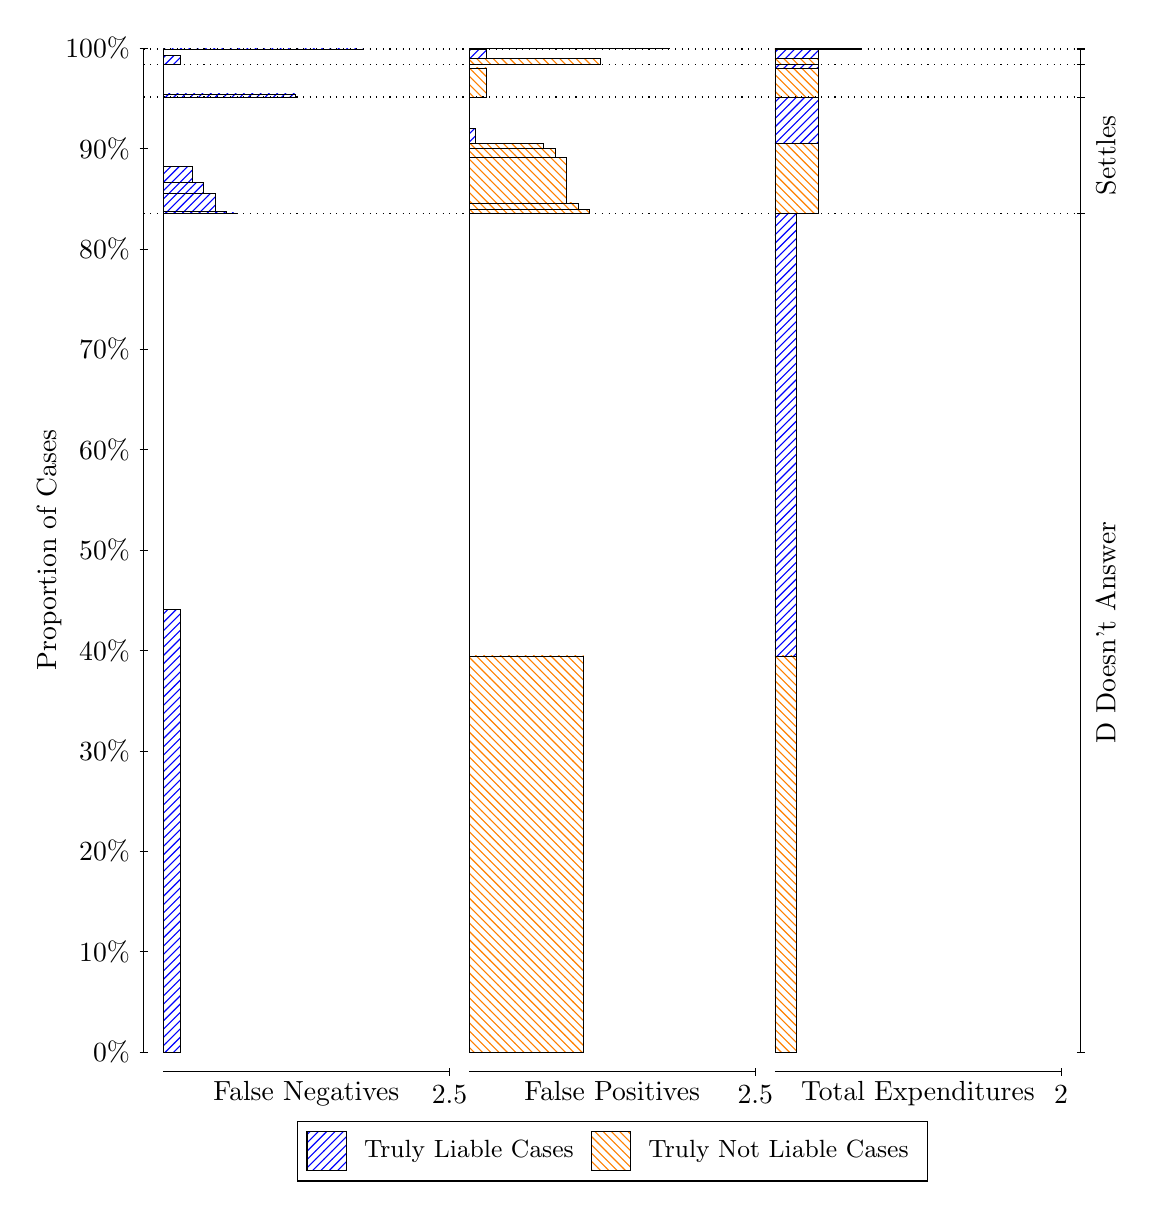
\begin{tikzpicture}
\draw[black, very thin] (1.5,1.75) -- (1.5,14.5);
\node[rotate=90, text=black, anchor=center] at (0.3, 8.125) {Proportion of Cases};
\draw[black, very thin] (1.45,1.75) -- (1.55,1.75);
\node[text=black, anchor=east] at (1.45, 1.75) {0\%};
\draw[black, very thin] (1.45,3.025) -- (1.55,3.025);
\node[text=black, anchor=east] at (1.45, 3.025) {10\%};
\draw[black, very thin] (1.45,4.3) -- (1.55,4.3);
\node[text=black, anchor=east] at (1.45, 4.3) {20\%};
\draw[black, very thin] (1.45,5.575) -- (1.55,5.575);
\node[text=black, anchor=east] at (1.45, 5.575) {30\%};
\draw[black, very thin] (1.45,6.85) -- (1.55,6.85);
\node[text=black, anchor=east] at (1.45, 6.85) {40\%};
\draw[black, very thin] (1.45,8.125) -- (1.55,8.125);
\node[text=black, anchor=east] at (1.45, 8.125) {50\%};
\draw[black, very thin] (1.45,9.4) -- (1.55,9.4);
\node[text=black, anchor=east] at (1.45, 9.4) {60\%};
\draw[black, very thin] (1.45,10.675) -- (1.55,10.675);
\node[text=black, anchor=east] at (1.45, 10.675) {70\%};
\draw[black, very thin] (1.45,11.95) -- (1.55,11.95);
\node[text=black, anchor=east] at (1.45, 11.95) {80\%};
\draw[black, very thin] (1.45,13.225) -- (1.55,13.225);
\node[text=black, anchor=east] at (1.45, 13.225) {90\%};
\draw[black, very thin] (1.45,14.5) -- (1.55,14.5);
\node[text=black, anchor=east] at (1.45, 14.5) {100\%};

\draw[black, very thin] (13.4,1.75) -- (13.4,14.5);
\draw[black, very thin] (13.35,1.75) -- (13.45,1.75);
\node[anchor=west] at (13.35, 1.75) {};
\draw[black, very thin] (13.35,12.4) -- (13.45,12.4);
\node[anchor=west] at (13.35, 12.4) {};
\draw[black, very thin] (13.35,13.878) -- (13.45,13.878);
\node[anchor=west] at (13.35, 13.878) {};
\draw[black, very thin] (13.35,14.29) -- (13.45,14.29);
\node[anchor=west] at (13.35, 14.29) {};
\draw[black, very thin] (13.35,14.486) -- (13.45,14.486);
\node[anchor=west] at (13.35, 14.486) {};
\draw[black, very thin] (13.35,14.495) -- (13.45,14.495);
\node[anchor=west] at (13.35, 14.495) {};
\draw[black, very thin] (13.35,14.5) -- (13.45,14.5);
\node[anchor=west] at (13.35, 14.5) {};

\draw[black, very thin, pattern color=blue, pattern=north east lines] (1.75,1.75) rectangle (1.968,7.3707);
\draw[black, very thin, pattern color=orange, pattern=north west lines] (1.75,7.3707) rectangle (1.75,12.4);
\draw[black, very thin, pattern color=blue, pattern=north east lines] (1.75,12.4) rectangle (2.6947,12.405);
\draw[black, very thin, pattern color=blue, pattern=north east lines] (1.75,12.405) rectangle (2.5493,12.421);
\draw[black, very thin, pattern color=blue, pattern=north east lines] (1.75,12.421) rectangle (2.404,12.654);
\draw[black, very thin, pattern color=blue, pattern=north east lines] (1.75,12.654) rectangle (2.2587,12.798);
\draw[black, very thin, pattern color=blue, pattern=north east lines] (1.75,12.798) rectangle (2.1133,12.993);
\draw[black, very thin, pattern color=orange, pattern=north west lines] (1.75,12.993) rectangle (1.75,13.878);
\draw[black, very thin, pattern color=blue, pattern=north east lines] (1.75,13.878) rectangle (3.4213,13.918);
\draw[black, very thin, pattern color=orange, pattern=north west lines] (1.75,13.918) rectangle (1.75,14.29);
\draw[black, very thin, pattern color=blue, pattern=north east lines] (1.75,14.29) rectangle (1.968,14.406);
\draw[black, very thin, pattern color=orange, pattern=north west lines] (1.75,14.406) rectangle (1.75,14.486);
\draw[black, very thin, pattern color=blue, pattern=north east lines] (1.75,14.486) rectangle (4.2933,14.488);
\draw[black, very thin, pattern color=orange, pattern=north west lines] (1.75,14.488) rectangle (1.75,14.495);
\draw[black, very thin, pattern color=orange, pattern=north west lines] (1.75,14.495) rectangle (1.75,14.498);
\draw[black, very thin, pattern color=blue, pattern=north east lines] (1.75,14.498) rectangle (1.75,14.5);
\draw[black, very thin, pattern color=orange, pattern=north west lines] (5.6333,1.75) rectangle (7.0867,6.7796);
\draw[black, very thin, pattern color=blue, pattern=north east lines] (5.6333,6.7796) rectangle (5.6333,12.4);
\draw[black, very thin, pattern color=orange, pattern=north west lines] (5.6333,12.4) rectangle (7.1593,12.448);
\draw[black, very thin, pattern color=orange, pattern=north west lines] (5.6333,12.448) rectangle (7.014,12.533);
\draw[black, very thin, pattern color=orange, pattern=north west lines] (5.6333,12.533) rectangle (6.8687,13.107);
\draw[black, very thin, pattern color=orange, pattern=north west lines] (5.6333,13.107) rectangle (6.7233,13.227);
\draw[black, very thin, pattern color=orange, pattern=north west lines] (5.6333,13.227) rectangle (6.578,13.285);
\draw[black, very thin, pattern color=blue, pattern=north east lines] (5.6333,13.285) rectangle (5.706,13.48);
\draw[black, very thin, pattern color=blue, pattern=north east lines] (5.6333,13.48) rectangle (5.6333,13.878);
\draw[black, very thin, pattern color=orange, pattern=north west lines] (5.6333,13.878) rectangle (5.8513,14.249);
\draw[black, very thin, pattern color=blue, pattern=north east lines] (5.6333,14.249) rectangle (5.6333,14.29);
\draw[black, very thin, pattern color=orange, pattern=north west lines] (5.6333,14.29) rectangle (7.3047,14.37);
\draw[black, very thin, pattern color=blue, pattern=north east lines] (5.6333,14.37) rectangle (5.8513,14.486);
\draw[black, very thin, pattern color=orange, pattern=north west lines] (5.6333,14.486) rectangle (5.6333,14.493);
\draw[black, very thin, pattern color=blue, pattern=north east lines] (5.6333,14.493) rectangle (5.6333,14.495);
\draw[black, very thin, pattern color=orange, pattern=north west lines] (5.6333,14.495) rectangle (8.1767,14.498);
\draw[black, very thin, pattern color=blue, pattern=north east lines] (5.6333,14.498) rectangle (6.7233,14.5);
\draw[black, very thin, pattern color=orange, pattern=north west lines] (9.5167,1.75) rectangle (9.7892,6.7796);
\draw[black, very thin, pattern color=blue, pattern=north east lines] (9.5167,6.7796) rectangle (9.7892,12.4);
\draw[black, very thin, pattern color=orange, pattern=north west lines] (9.5167,12.4) rectangle (10.062,13.285);
\draw[black, very thin, pattern color=blue, pattern=north east lines] (9.5167,13.285) rectangle (10.062,13.878);
\draw[black, very thin, pattern color=orange, pattern=north west lines] (9.5167,13.878) rectangle (10.062,14.249);
\draw[black, very thin, pattern color=blue, pattern=north east lines] (9.5167,14.249) rectangle (10.062,14.29);
\draw[black, very thin, pattern color=orange, pattern=north west lines] (9.5167,14.29) rectangle (10.062,14.37);
\draw[black, very thin, pattern color=blue, pattern=north east lines] (9.5167,14.37) rectangle (10.062,14.486);
\draw[black, very thin, pattern color=orange, pattern=north west lines] (9.5167,14.486) rectangle (10.607,14.493);
\draw[black, very thin, pattern color=blue, pattern=north east lines] (9.5167,14.493) rectangle (10.607,14.495);
\draw[black, very thin, pattern color=orange, pattern=north west lines] (9.5167,14.495) rectangle (10.607,14.498);
\draw[black, very thin, pattern color=blue, pattern=north east lines] (9.5167,14.498) rectangle (10.607,14.5);
\draw[black, dotted] (1.5,12.4) -- (13.4,12.4);
\draw[black, dotted] (1.5,13.878) -- (13.4,13.878);
\draw[black, dotted] (1.5,14.29) -- (13.4,14.29);
\draw[black, dotted] (1.5,14.486) -- (13.4,14.486);
\draw[black, dotted] (1.5,14.495) -- (13.4,14.495);
\draw[black, very thin] (1.75,1.5) -- (5.3833,1.5);
\node[text=black, anchor=north] at (3.5667, 1.5) {False Negatives};
\draw[black, very thin] (5.3833,1.45) -- (5.3833,1.55);
\node[text=black, anchor=north] at (5.3833, 1.45) {2.5};

\draw[black, very thin] (5.6333,1.5) -- (9.2667,1.5);
\node[text=black, anchor=north] at (7.45, 1.5) {False Positives};
\draw[black, very thin] (9.2667,1.45) -- (9.2667,1.55);
\node[text=black, anchor=north] at (9.2667, 1.45) {2.5};

\draw[black, very thin] (9.5167,1.5) -- (13.15,1.5);
\node[text=black, anchor=north] at (11.333, 1.5) {Total Expenditures};
\draw[black, very thin] (13.15,1.45) -- (13.15,1.55);
\node[text=black, anchor=north] at (13.15, 1.45) {2};

\node[text=black, centered, rotate=90] at (13.72, 7.0752) {D Doesn't Answer};
\node[text=black, centered, rotate=90] at (13.72, 13.139) {Settles};





\draw (7.449999999999999,1.5) node[draw=none] (baseCoordinate) {};
\begin{scope}[align=center]
        \matrix[scale=0.5, draw=black, below=0.5cm of baseCoordinate, nodes={draw}, column sep=0.1cm]{
            \node[rectangle, draw, minimum width=0.5cm, minimum height=0.5cm, pattern color=blue, pattern=north east lines] {}; &
            \node[draw=none, font=\small, text=black] (B) {Truly Liable Cases}; &
            \node[rectangle, draw, minimum width=0.5cm, minimum height=0.5cm, pattern color=orange, pattern=north west lines] {}; &
            \node[draw=none, font=\small, text=black] (B) {Truly Not Liable Cases}; \\
            };
\end{scope}

\end{tikzpicture}
\end{document}